\documentclass[1p]{elsarticle_modified}
%\bibliographystyle{elsarticle-num}

%\usepackage[colorlinks]{hyperref}
%\usepackage{abbrmath_seonhwa} %\Abb, \Ascr, \Acal ,\Abf, \Afrak
\usepackage{amsfonts}
\usepackage{amssymb}
\usepackage{amsmath}
\usepackage{amsthm}
\usepackage{scalefnt}
\usepackage{amsbsy}
\usepackage{kotex}
\usepackage{caption}
\usepackage{subfig}
\usepackage{color}
\usepackage{graphicx}
\usepackage{xcolor} %% white, black, red, green, blue, cyan, magenta, yellow
\usepackage{float}
\usepackage{setspace}
\usepackage{hyperref}

\usepackage{tikz}
\usetikzlibrary{arrows}

\usepackage{multirow}
\usepackage{array} % fixed length table
\usepackage{hhline}

%%%%%%%%%%%%%%%%%%%%%
\makeatletter
\renewcommand*\env@matrix[1][\arraystretch]{%
	\edef\arraystretch{#1}%
	\hskip -\arraycolsep
	\let\@ifnextchar\new@ifnextchar
	\array{*\c@MaxMatrixCols c}}
\makeatother %https://tex.stackexchange.com/questions/14071/how-can-i-increase-the-line-spacing-in-a-matrix
%%%%%%%%%%%%%%%

\usepackage[normalem]{ulem}

\newcommand{\msout}[1]{\ifmmode\text{\sout{\ensuremath{#1}}}\else\sout{#1}\fi}
%SOURCE: \msout is \stkout macro in https://tex.stackexchange.com/questions/20609/strikeout-in-math-mode

\newcommand{\cancel}[1]{
	\ifmmode
	{\color{red}\msout{#1}}
	\else
	{\color{red}\sout{#1}}
	\fi
}

\newcommand{\add}[1]{
	{\color{blue}\uwave{#1}}
}

\newcommand{\replace}[2]{
	\ifmmode
	{\color{red}\msout{#1}}{\color{blue}\uwave{#2}}
	\else
	{\color{red}\sout{#1}}{\color{blue}\uwave{#2}}
	\fi
}

\newcommand{\Sol}{\mathcal{S}} %segment
\newcommand{\D}{D} %diagram
\newcommand{\A}{\mathcal{A}} %arc


%%%%%%%%%%%%%%%%%%%%%%%%%%%%%5 test

\def\sl{\operatorname{\textup{SL}}(2,\Cbb)}
\def\psl{\operatorname{\textup{PSL}}(2,\Cbb)}
\def\quan{\mkern 1mu \triangleright \mkern 1mu}

\theoremstyle{definition}
\newtheorem{thm}{Theorem}[section]
\newtheorem{prop}[thm]{Proposition}
\newtheorem{lem}[thm]{Lemma}
\newtheorem{ques}[thm]{Question}
\newtheorem{cor}[thm]{Corollary}
\newtheorem{defn}[thm]{Definition}
\newtheorem{exam}[thm]{Example}
\newtheorem{rmk}[thm]{Remark}
\newtheorem{alg}[thm]{Algorithm}

\newcommand{\I}{\sqrt{-1}}
\begin{document}

%\begin{frontmatter}
%
%\title{Boundary parabolic representations of knots up to 8 crossings}
%
%%% Group authors per affiliation:
%\author{Yunhi Cho} 
%\address{Department of Mathematics, University of Seoul, Seoul, Korea}
%\ead{yhcho@uos.ac.kr}
%
%
%\author{Seonhwa Kim} %\fnref{s_kim}}
%\address{Center for Geometry and Physics, Institute for Basic Science, Pohang, 37673, Korea}
%\ead{ryeona17@ibs.re.kr}
%
%\author{Hyuk Kim}
%\address{Department of Mathematical Sciences, Seoul National University, Seoul 08826, Korea}
%\ead{hyukkim@snu.ac.kr}
%
%\author{Seokbeom Yoon}
%\address{Department of Mathematical Sciences, Seoul National University, Seoul, 08826,  Korea}
%\ead{sbyoon15@snu.ac.kr}
%
%\begin{abstract}
%We find all boundary parabolic representation of knots up to 8 crossings.
%
%\end{abstract}
%\begin{keyword}
%    \MSC[2010] 57M25 
%\end{keyword}
%
%\end{frontmatter}

%\linenumbers
%\tableofcontents
%
\newcommand\colored[1]{\textcolor{white}{\rule[-0.35ex]{0.8em}{1.4ex}}\kern-0.8em\color{red} #1}%
%\newcommand\colored[1]{\textcolor{white}{ #1}\kern-2.17ex	\textcolor{white}{ #1}\kern-1.81ex	\textcolor{white}{ #1}\kern-2.15ex\color{red}#1	}

{\Large $\underline{12a_{0289}~(K12a_{0289})}$}

\setlength{\tabcolsep}{10pt}
\renewcommand{\arraystretch}{1.6}
\vspace{1cm}\begin{tabular}{m{100pt}>{\centering\arraybackslash}m{274pt}}
\multirow{5}{120pt}{
	\centering
	\includegraphics[width=112pt]{../../../GIT/diagram.site/Diagrams/png/1090_12a_0289.png}\\
\ \ \ A knot diagram\footnotemark}&
\allowdisplaybreaks
\textbf{Linearized knot diagam} \\
\cline{2-2}
 &
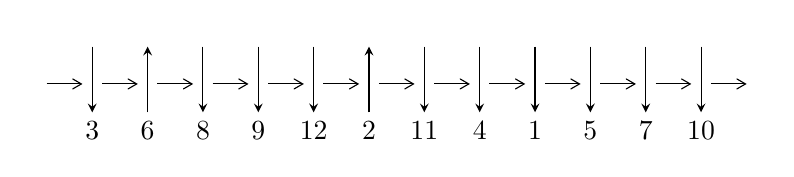
\begin{tikzpicture}[x=20pt, y=17pt]
	% nodes
	\node (C0) at (0, 0) {};
	\node (C1) at (1, 0) {};
	\node (C1U) at (1, +1) {};
	\node (C1D) at (1, -1) {3};

	\node (C2) at (2, 0) {};
	\node (C2U) at (2, +1) {};
	\node (C2D) at (2, -1) {6};

	\node (C3) at (3, 0) {};
	\node (C3U) at (3, +1) {};
	\node (C3D) at (3, -1) {8};

	\node (C4) at (4, 0) {};
	\node (C4U) at (4, +1) {};
	\node (C4D) at (4, -1) {9};

	\node (C5) at (5, 0) {};
	\node (C5U) at (5, +1) {};
	\node (C5D) at (5, -1) {12};

	\node (C6) at (6, 0) {};
	\node (C6U) at (6, +1) {};
	\node (C6D) at (6, -1) {2};

	\node (C7) at (7, 0) {};
	\node (C7U) at (7, +1) {};
	\node (C7D) at (7, -1) {11};

	\node (C8) at (8, 0) {};
	\node (C8U) at (8, +1) {};
	\node (C8D) at (8, -1) {4};

	\node (C9) at (9, 0) {};
	\node (C9U) at (9, +1) {};
	\node (C9D) at (9, -1) {1};

	\node (C10) at (10, 0) {};
	\node (C10U) at (10, +1) {};
	\node (C10D) at (10, -1) {5};

	\node (C11) at (11, 0) {};
	\node (C11U) at (11, +1) {};
	\node (C11D) at (11, -1) {7};

	\node (C12) at (12, 0) {};
	\node (C12U) at (12, +1) {};
	\node (C12D) at (12, -1) {10};
	\node (C13) at (13, 0) {};

	% arrows
	\draw[->,>={angle 60}]
	(C0) edge (C1) (C1) edge (C2) (C2) edge (C3) (C3) edge (C4) (C4) edge (C5) (C5) edge (C6) (C6) edge (C7) (C7) edge (C8) (C8) edge (C9) (C9) edge (C10) (C10) edge (C11) (C11) edge (C12) (C12) edge (C13) ;	\draw[->,>=stealth]
	(C1U) edge (C1D) (C2D) edge (C2U) (C3U) edge (C3D) (C4U) edge (C4D) (C5U) edge (C5D) (C6D) edge (C6U) (C7U) edge (C7D) (C8U) edge (C8D) (C9U) edge (C9D) (C10U) edge (C10D) (C11U) edge (C11D) (C12U) edge (C12D) ;
	\end{tikzpicture} \\
\hhline{~~} \\& 
\textbf{Solving Sequence} \\ \cline{2-2} 
 &
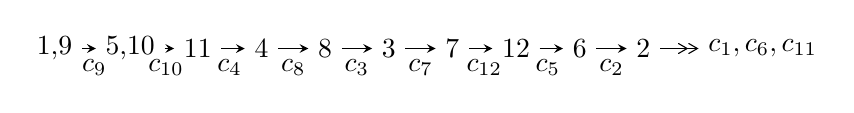
\begin{tikzpicture}[x=23pt, y=7pt]
	% node
	\node (A0) at (-1/8, 0) {1,9};
	\node (A1) at (17/16, 0) {5,10};
	\node (A2) at (17/8, 0) {11};
	\node (A3) at (25/8, 0) {4};
	\node (A4) at (33/8, 0) {8};
	\node (A5) at (41/8, 0) {3};
	\node (A6) at (49/8, 0) {7};
	\node (A7) at (57/8, 0) {12};
	\node (A8) at (65/8, 0) {6};
	\node (A9) at (73/8, 0) {2};
	\node (C1) at (1/2, -1) {$c_{9}$};
	\node (C2) at (13/8, -1) {$c_{10}$};
	\node (C3) at (21/8, -1) {$c_{4}$};
	\node (C4) at (29/8, -1) {$c_{8}$};
	\node (C5) at (37/8, -1) {$c_{3}$};
	\node (C6) at (45/8, -1) {$c_{7}$};
	\node (C7) at (53/8, -1) {$c_{12}$};
	\node (C8) at (61/8, -1) {$c_{5}$};
	\node (C9) at (69/8, -1) {$c_{2}$};
	\node (A10) at (11, 0) {$c_{1},c_{6},c_{11}$};

	% edge
	\draw[->,>=stealth]	
	(A0) edge (A1) (A1) edge (A2) (A2) edge (A3) (A3) edge (A4) (A4) edge (A5) (A5) edge (A6) (A6) edge (A7) (A7) edge (A8) (A8) edge (A9) ;
	\draw[->>,>={angle 60}]	
	(A9) edge (A10);
\end{tikzpicture} \\ 

\end{tabular} \\

\footnotetext{
The image of knot diagram is generated by the software ``\textbf{Draw programme}" developed by Andrew Bartholomew(\url{http://www.layer8.co.uk/maths/draw/index.htm\#Running-draw}), where we modified some parts for our purpose(\url{https://github.com/CATsTAILs/LinksPainter}).
}\phantom \\ \newline 
\centering \textbf{Ideals for irreducible components\footnotemark of $X_{\text{par}}$} 
 
\begin{align*}
I^u_{1}&=\langle 
1.23054\times10^{549} u^{129}+7.13939\times10^{549} u^{128}+\cdots+1.47559\times10^{551} b-4.80171\times10^{551},\\
\phantom{I^u_{1}}&\phantom{= \langle  }-2.58879\times10^{552} u^{129}-1.24968\times10^{553} u^{128}+\cdots+4.53005\times10^{553} a-4.77775\times10^{555},\\
\phantom{I^u_{1}}&\phantom{= \langle  }u^{130}+5 u^{129}+\cdots+9370 u+307\rangle \\
I^u_{2}&=\langle 
9059013 u^{33}-52630678 u^{32}+\cdots+321857 b-3891846,\\
\phantom{I^u_{2}}&\phantom{= \langle  }-9774026 u^{33}+58589548 u^{32}+\cdots+321857 a+3891173,\;u^{34}-6 u^{33}+\cdots-6 u+1\rangle \\
\\
\end{align*}
\raggedright * 2 irreducible components of $\dim_{\mathbb{C}}=0$, with total 164 representations.\\
\footnotetext{All coefficients of polynomials are rational numbers. But the coefficients are sometimes approximated in decimal forms when there is not enough margin.}
\newpage
\renewcommand{\arraystretch}{1}
\centering \section*{I. $I^u_{1}= \langle 1.23\times10^{549} u^{129}+7.14\times10^{549} u^{128}+\cdots+1.48\times10^{551} b-4.80\times10^{551},\;-2.59\times10^{552} u^{129}-1.25\times10^{553} u^{128}+\cdots+4.53\times10^{553} a-4.78\times10^{555},\;u^{130}+5 u^{129}+\cdots+9370 u+307 \rangle$}
\flushleft \textbf{(i) Arc colorings}\\
\begin{tabular}{m{7pt} m{180pt} m{7pt} m{180pt} }
\flushright $a_{1}=$&$\begin{pmatrix}0\\u\end{pmatrix}$ \\
\flushright $a_{9}=$&$\begin{pmatrix}1\\0\end{pmatrix}$ \\
\flushright $a_{5}=$&$\begin{pmatrix}0.0571471 u^{129}+0.275864 u^{128}+\cdots+2416.99 u+105.468\\-0.00833933 u^{129}-0.0483834 u^{128}+\cdots+10.4028 u+3.25410\end{pmatrix}$ \\
\flushright $a_{10}=$&$\begin{pmatrix}1\\u^2\end{pmatrix}$ \\
\flushright $a_{11}=$&$\begin{pmatrix}0.0424528 u^{129}+0.203895 u^{128}+\cdots+1460.64 u+58.0744\\-0.0287762 u^{129}-0.130522 u^{128}+\cdots+107.795 u+4.49195\end{pmatrix}$ \\
\flushright $a_{4}=$&$\begin{pmatrix}0.0488078 u^{129}+0.227480 u^{128}+\cdots+2427.40 u+108.722\\-0.00833933 u^{129}-0.0483834 u^{128}+\cdots+10.4028 u+3.25410\end{pmatrix}$ \\
\flushright $a_{8}=$&$\begin{pmatrix}-0.0257256 u^{129}-0.125360 u^{128}+\cdots-1959.45 u-75.4831\\0.0164267 u^{129}+0.0571151 u^{128}+\cdots-359.900 u-13.1760\end{pmatrix}$ \\
\flushright $a_{3}=$&$\begin{pmatrix}0.0340470 u^{129}+0.157222 u^{128}+\cdots+2386.50 u+110.752\\0.0197080 u^{129}+0.138612 u^{128}+\cdots+995.383 u+36.2377\end{pmatrix}$ \\
\flushright $a_{7}=$&$\begin{pmatrix}-0.0342572 u^{129}-0.172968 u^{128}+\cdots-1101.16 u-43.1706\\0.000292252 u^{129}-0.0153436 u^{128}+\cdots-265.849 u-9.05471\end{pmatrix}$ \\
\flushright $a_{12}=$&$\begin{pmatrix}u\\u^3+u\end{pmatrix}$ \\
\flushright $a_{6}=$&$\begin{pmatrix}0.0548184 u^{129}+0.255512 u^{128}+\cdots+2336.78 u+103.311\\-0.000327503 u^{129}-0.0231974 u^{128}+\cdots+12.5010 u+3.77093\end{pmatrix}$ \\
\flushright $a_{2}=$&$\begin{pmatrix}-0.00945379 u^{129}-0.0396822 u^{128}+\cdots+1855.44 u+87.3425\\-0.00862843 u^{129}-0.0542862 u^{128}+\cdots+355.882 u+14.9677\end{pmatrix}$\\&\end{tabular}
\flushleft \textbf{(ii) Obstruction class $= -1$}\\~\\
\flushleft \textbf{(iii) Cusp Shapes $= -0.165409 u^{129}-0.885526 u^{128}+\cdots-1219.93 u-34.2034$}\\~\\
\newpage\renewcommand{\arraystretch}{1}
\flushleft \textbf{(iv) u-Polynomials at the component}\newline \\
\begin{tabular}{m{50pt}|m{274pt}}
Crossings & \hspace{64pt}u-Polynomials at each crossing \\
\hline $$\begin{aligned}c_{1}\end{aligned}$$&$\begin{aligned}
&u^{130}+54 u^{129}+\cdots-5575 u+7921
\end{aligned}$\\
\hline $$\begin{aligned}c_{2},c_{6}\end{aligned}$$&$\begin{aligned}
&u^{130}+27 u^{128}+\cdots-71 u-89
\end{aligned}$\\
\hline $$\begin{aligned}c_{3},c_{4},c_{8}\end{aligned}$$&$\begin{aligned}
&u^{130}- u^{129}+\cdots+4476 u-653
\end{aligned}$\\
\hline $$\begin{aligned}c_{5}\end{aligned}$$&$\begin{aligned}
&u^{130}- u^{129}+\cdots-5193796 u-5692175
\end{aligned}$\\
\hline $$\begin{aligned}c_{7},c_{11}\end{aligned}$$&$\begin{aligned}
&u^{130}+3 u^{129}+\cdots-119574 u-21673
\end{aligned}$\\
\hline $$\begin{aligned}c_{9},c_{12}\end{aligned}$$&$\begin{aligned}
&u^{130}-5 u^{129}+\cdots-9370 u+307
\end{aligned}$\\
\hline $$\begin{aligned}c_{10}\end{aligned}$$&$\begin{aligned}
&u^{130}+u^{129}+\cdots-263540 u-65057
\end{aligned}$\\
\hline
\end{tabular}\\~\\
\newpage\renewcommand{\arraystretch}{1}
\flushleft \textbf{(v) Riley Polynomials at the component}\newline \\
\begin{tabular}{m{50pt}|m{274pt}}
Crossings & \hspace{64pt}Riley Polynomials at each crossing \\
\hline $$\begin{aligned}c_{1}\end{aligned}$$&$\begin{aligned}
&y^{130}+62 y^{129}+\cdots-19593843639 y+62742241
\end{aligned}$\\
\hline $$\begin{aligned}c_{2},c_{6}\end{aligned}$$&$\begin{aligned}
&y^{130}+54 y^{129}+\cdots-5575 y+7921
\end{aligned}$\\
\hline $$\begin{aligned}c_{3},c_{4},c_{8}\end{aligned}$$&$\begin{aligned}
&y^{130}-123 y^{129}+\cdots+2757736 y+426409
\end{aligned}$\\
\hline $$\begin{aligned}c_{5}\end{aligned}$$&$\begin{aligned}
&y^{130}+49 y^{129}+\cdots+915788440159684 y+32400856230625
\end{aligned}$\\
\hline $$\begin{aligned}c_{7},c_{11}\end{aligned}$$&$\begin{aligned}
&y^{130}+83 y^{129}+\cdots+11741041028 y+469718929
\end{aligned}$\\
\hline $$\begin{aligned}c_{9},c_{12}\end{aligned}$$&$\begin{aligned}
&y^{130}+75 y^{129}+\cdots-8845710 y+94249
\end{aligned}$\\
\hline $$\begin{aligned}c_{10}\end{aligned}$$&$\begin{aligned}
&y^{130}+13 y^{129}+\cdots+211632593170 y+4232413249
\end{aligned}$\\
\hline
\end{tabular}\\~\\
\newpage\flushleft \textbf{(vi) Complex Volumes and Cusp Shapes}
$$\begin{array}{c|c|c}  
\text{Solutions to }I^u_{1}& \I (\text{vol} + \sqrt{-1}CS) & \text{Cusp shape}\\
 \hline 
\begin{aligned}
u &= -0.998922 + 0.037072 I \\
a &= -0.251102 - 0.217828 I \\
b &= \phantom{-}0.310908 + 0.713630 I\end{aligned}
 & \phantom{-}2.66752 - 8.25962 I & \phantom{-0.000000 } 0 \\ \hline\begin{aligned}
u &= -0.998922 - 0.037072 I \\
a &= -0.251102 + 0.217828 I \\
b &= \phantom{-}0.310908 - 0.713630 I\end{aligned}
 & \phantom{-}2.66752 + 8.25962 I & \phantom{-0.000000 } 0 \\ \hline\begin{aligned}
u &= \phantom{-}0.488004 + 0.876844 I \\
a &= \phantom{-}0.567135 - 1.192750 I \\
b &= -0.231263 + 0.957518 I\end{aligned}
 & \phantom{-}1.80629 + 0.07312 I & \phantom{-0.000000 } 0 \\ \hline\begin{aligned}
u &= \phantom{-}0.488004 - 0.876844 I \\
a &= \phantom{-}0.567135 + 1.192750 I \\
b &= -0.231263 - 0.957518 I\end{aligned}
 & \phantom{-}1.80629 - 0.07312 I & \phantom{-0.000000 } 0 \\ \hline\begin{aligned}
u &= -0.373524 + 0.931545 I \\
a &= -0.28618 + 1.53825 I \\
b &= \phantom{-}1.348360 - 0.231599 I\end{aligned}
 & -2.03553 + 1.90796 I & \phantom{-0.000000 } 0 \\ \hline\begin{aligned}
u &= -0.373524 - 0.931545 I \\
a &= -0.28618 - 1.53825 I \\
b &= \phantom{-}1.348360 + 0.231599 I\end{aligned}
 & -2.03553 - 1.90796 I & \phantom{-0.000000 } 0 \\ \hline\begin{aligned}
u &= \phantom{-}0.180247 + 0.989091 I \\
a &= \phantom{-}1.31579 - 1.95264 I \\
b &= \phantom{-}1.42664 + 0.15993 I\end{aligned}
 & \phantom{-}0.14796 - 7.11169 I & \phantom{-0.000000 } 0 \\ \hline\begin{aligned}
u &= \phantom{-}0.180247 - 0.989091 I \\
a &= \phantom{-}1.31579 + 1.95264 I \\
b &= \phantom{-}1.42664 - 0.15993 I\end{aligned}
 & \phantom{-}0.14796 + 7.11169 I & \phantom{-0.000000 } 0 \\ \hline\begin{aligned}
u &= -0.420327 + 0.915445 I \\
a &= \phantom{-}0.14191 - 1.81983 I \\
b &= -1.49832 + 0.32981 I\end{aligned}
 & -5.54583 + 6.41365 I & \phantom{-0.000000 } 0 \\ \hline\begin{aligned}
u &= -0.420327 - 0.915445 I \\
a &= \phantom{-}0.14191 + 1.81983 I \\
b &= -1.49832 - 0.32981 I\end{aligned}
 & -5.54583 - 6.41365 I & \phantom{-0.000000 } 0\\
 \hline 
 \end{array}$$\newpage$$\begin{array}{c|c|c}  
\text{Solutions to }I^u_{1}& \I (\text{vol} + \sqrt{-1}CS) & \text{Cusp shape}\\
 \hline 
\begin{aligned}
u &= -0.626447 + 0.760676 I \\
a &= \phantom{-}1.10415 + 1.42302 I \\
b &= \phantom{-}0.965108 + 0.018640 I\end{aligned}
 & \phantom{-}1.42300 + 4.98117 I & \phantom{-0.000000 } 0 \\ \hline\begin{aligned}
u &= -0.626447 - 0.760676 I \\
a &= \phantom{-}1.10415 - 1.42302 I \\
b &= \phantom{-}0.965108 - 0.018640 I\end{aligned}
 & \phantom{-}1.42300 - 4.98117 I & \phantom{-0.000000 } 0 \\ \hline\begin{aligned}
u &= \phantom{-}0.080531 + 0.979351 I \\
a &= \phantom{-}0.12418 + 2.65907 I \\
b &= -1.278130 - 0.144203 I\end{aligned}
 & \phantom{-}3.58342 - 0.34128 I & \phantom{-0.000000 } 0 \\ \hline\begin{aligned}
u &= \phantom{-}0.080531 - 0.979351 I \\
a &= \phantom{-}0.12418 - 2.65907 I \\
b &= -1.278130 + 0.144203 I\end{aligned}
 & \phantom{-}3.58342 + 0.34128 I & \phantom{-0.000000 } 0 \\ \hline\begin{aligned}
u &= \phantom{-}0.126615 + 1.026830 I \\
a &= -0.091407 - 1.342550 I \\
b &= -0.022685 + 0.760118 I\end{aligned}
 & \phantom{-}2.31765 - 1.53047 I & \phantom{-0.000000 } 0 \\ \hline\begin{aligned}
u &= \phantom{-}0.126615 - 1.026830 I \\
a &= -0.091407 + 1.342550 I \\
b &= -0.022685 - 0.760118 I\end{aligned}
 & \phantom{-}2.31765 + 1.53047 I & \phantom{-0.000000 } 0 \\ \hline\begin{aligned}
u &= \phantom{-}0.270875 + 1.001640 I \\
a &= -1.31017 - 1.36501 I \\
b &= \phantom{-}1.39537 + 0.33356 I\end{aligned}
 & -4.33445 - 2.90226 I & \phantom{-0.000000 } 0 \\ \hline\begin{aligned}
u &= \phantom{-}0.270875 - 1.001640 I \\
a &= -1.31017 + 1.36501 I \\
b &= \phantom{-}1.39537 - 0.33356 I\end{aligned}
 & -4.33445 + 2.90226 I & \phantom{-0.000000 } 0 \\ \hline\begin{aligned}
u &= \phantom{-}0.466298 + 0.929511 I \\
a &= -0.205508 + 1.271420 I \\
b &= -0.211418 - 0.257274 I\end{aligned}
 & -1.41170 - 2.59593 I & \phantom{-0.000000 } 0 \\ \hline\begin{aligned}
u &= \phantom{-}0.466298 - 0.929511 I \\
a &= -0.205508 - 1.271420 I \\
b &= -0.211418 + 0.257274 I\end{aligned}
 & -1.41170 + 2.59593 I & \phantom{-0.000000 } 0\\
 \hline 
 \end{array}$$\newpage$$\begin{array}{c|c|c}  
\text{Solutions to }I^u_{1}& \I (\text{vol} + \sqrt{-1}CS) & \text{Cusp shape}\\
 \hline 
\begin{aligned}
u &= \phantom{-}0.800134 + 0.522066 I \\
a &= -0.026229 - 0.197610 I \\
b &= -0.483920 + 0.094949 I\end{aligned}
 & -2.63126 - 2.06050 I & \phantom{-0.000000 } 0 \\ \hline\begin{aligned}
u &= \phantom{-}0.800134 - 0.522066 I \\
a &= -0.026229 + 0.197610 I \\
b &= -0.483920 - 0.094949 I\end{aligned}
 & -2.63126 + 2.06050 I & \phantom{-0.000000 } 0 \\ \hline\begin{aligned}
u &= -0.339304 + 0.884538 I \\
a &= \phantom{-}0.83930 - 1.61458 I \\
b &= -1.43241 + 0.06380 I\end{aligned}
 & -5.64729 - 2.34449 I & \phantom{-0.000000 } 0 \\ \hline\begin{aligned}
u &= -0.339304 - 0.884538 I \\
a &= \phantom{-}0.83930 + 1.61458 I \\
b &= -1.43241 - 0.06380 I\end{aligned}
 & -5.64729 + 2.34449 I & \phantom{-0.000000 } 0 \\ \hline\begin{aligned}
u &= \phantom{-}0.854041 + 0.406562 I \\
a &= \phantom{-}0.073292 + 0.125300 I \\
b &= -1.339470 + 0.246472 I\end{aligned}
 & -3.53513 - 0.33068 I & \phantom{-0.000000 } 0 \\ \hline\begin{aligned}
u &= \phantom{-}0.854041 - 0.406562 I \\
a &= \phantom{-}0.073292 - 0.125300 I \\
b &= -1.339470 - 0.246472 I\end{aligned}
 & -3.53513 + 0.33068 I & \phantom{-0.000000 } 0 \\ \hline\begin{aligned}
u &= \phantom{-}0.959676 + 0.497536 I \\
a &= \phantom{-}0.651009 + 0.038021 I \\
b &= \phantom{-}1.46933 - 0.03010 I\end{aligned}
 & -9.03057 - 1.52462 I & \phantom{-0.000000 } 0 \\ \hline\begin{aligned}
u &= \phantom{-}0.959676 - 0.497536 I \\
a &= \phantom{-}0.651009 - 0.038021 I \\
b &= \phantom{-}1.46933 + 0.03010 I\end{aligned}
 & -9.03057 + 1.52462 I & \phantom{-0.000000 } 0 \\ \hline\begin{aligned}
u &= \phantom{-}0.665755 + 0.625383 I \\
a &= -0.208885 - 0.017185 I \\
b &= \phantom{-}1.45889 - 0.31567 I\end{aligned}
 & -3.84118 + 4.56251 I & \phantom{-0.000000 } 0 \\ \hline\begin{aligned}
u &= \phantom{-}0.665755 - 0.625383 I \\
a &= -0.208885 + 0.017185 I \\
b &= \phantom{-}1.45889 + 0.31567 I\end{aligned}
 & -3.84118 - 4.56251 I & \phantom{-0.000000 } 0\\
 \hline 
 \end{array}$$\newpage$$\begin{array}{c|c|c}  
\text{Solutions to }I^u_{1}& \I (\text{vol} + \sqrt{-1}CS) & \text{Cusp shape}\\
 \hline 
\begin{aligned}
u &= -0.373694 + 1.024360 I \\
a &= -0.875919 - 0.950000 I \\
b &= \phantom{-}0.556664 + 0.865976 I\end{aligned}
 & \phantom{-}1.59255 + 0.75713 I & \phantom{-0.000000 } 0 \\ \hline\begin{aligned}
u &= -0.373694 - 1.024360 I \\
a &= -0.875919 + 0.950000 I \\
b &= \phantom{-}0.556664 - 0.865976 I\end{aligned}
 & \phantom{-}1.59255 - 0.75713 I & \phantom{-0.000000 } 0 \\ \hline\begin{aligned}
u &= -0.508519 + 0.746264 I \\
a &= \phantom{-}0.231386 - 0.933285 I \\
b &= -1.52146 - 0.13241 I\end{aligned}
 & -6.06120 - 2.63244 I & \phantom{-0.000000 } 0 \\ \hline\begin{aligned}
u &= -0.508519 - 0.746264 I \\
a &= \phantom{-}0.231386 + 0.933285 I \\
b &= -1.52146 + 0.13241 I\end{aligned}
 & -6.06120 + 2.63244 I & \phantom{-0.000000 } 0 \\ \hline\begin{aligned}
u &= \phantom{-}0.569803 + 0.943381 I \\
a &= -0.31490 - 1.94072 I \\
b &= \phantom{-}1.36946 + 0.47259 I\end{aligned}
 & -2.90017 - 9.35280 I & \phantom{-0.000000 } 0 \\ \hline\begin{aligned}
u &= \phantom{-}0.569803 - 0.943381 I \\
a &= -0.31490 + 1.94072 I \\
b &= \phantom{-}1.36946 - 0.47259 I\end{aligned}
 & -2.90017 + 9.35280 I & \phantom{-0.000000 } 0 \\ \hline\begin{aligned}
u &= -0.888534 + 0.104450 I \\
a &= \phantom{-}0.305653 - 0.332211 I \\
b &= -0.301474 + 0.590297 I\end{aligned}
 & \phantom{-}4.08616 + 2.89825 I & \phantom{-0.000000 } 0 \\ \hline\begin{aligned}
u &= -0.888534 - 0.104450 I \\
a &= \phantom{-}0.305653 + 0.332211 I \\
b &= -0.301474 - 0.590297 I\end{aligned}
 & \phantom{-}4.08616 - 2.89825 I & \phantom{-0.000000 } 0 \\ \hline\begin{aligned}
u &= -0.375206 + 0.778037 I \\
a &= \phantom{-}1.44735 + 0.67352 I \\
b &= -0.584094 - 0.076342 I\end{aligned}
 & \phantom{-}4.20952 + 1.45294 I & \phantom{-0.000000 } 0 \\ \hline\begin{aligned}
u &= -0.375206 - 0.778037 I \\
a &= \phantom{-}1.44735 - 0.67352 I \\
b &= -0.584094 + 0.076342 I\end{aligned}
 & \phantom{-}4.20952 - 1.45294 I & \phantom{-0.000000 } 0\\
 \hline 
 \end{array}$$\newpage$$\begin{array}{c|c|c}  
\text{Solutions to }I^u_{1}& \I (\text{vol} + \sqrt{-1}CS) & \text{Cusp shape}\\
 \hline 
\begin{aligned}
u &= \phantom{-}1.13859\phantom{ +0.000000I} \\
a &= -0.382090\phantom{ +0.000000I} \\
b &= -1.34469\phantom{ +0.000000I}\end{aligned}
 & -5.92828\phantom{ +0.000000I} & \phantom{-0.000000 } 0 \\ \hline\begin{aligned}
u &= \phantom{-}0.177435 + 0.841260 I \\
a &= -1.08968 - 3.21917 I \\
b &= \phantom{-}1.243330 - 0.036580 I\end{aligned}
 & -0.36112 + 5.47662 I & \phantom{-0.000000 } 0 \\ \hline\begin{aligned}
u &= \phantom{-}0.177435 - 0.841260 I \\
a &= -1.08968 + 3.21917 I \\
b &= \phantom{-}1.243330 + 0.036580 I\end{aligned}
 & -0.36112 - 5.47662 I & \phantom{-0.000000 } 0 \\ \hline\begin{aligned}
u &= \phantom{-}0.073243 + 1.145020 I \\
a &= -0.064810 + 1.040970 I \\
b &= \phantom{-}0.741472 - 0.620426 I\end{aligned}
 & \phantom{-}2.38171 + 1.93938 I & \phantom{-0.000000 } 0 \\ \hline\begin{aligned}
u &= \phantom{-}0.073243 - 1.145020 I \\
a &= -0.064810 - 1.040970 I \\
b &= \phantom{-}0.741472 + 0.620426 I\end{aligned}
 & \phantom{-}2.38171 - 1.93938 I & \phantom{-0.000000 } 0 \\ \hline\begin{aligned}
u &= -0.402200 + 1.075800 I \\
a &= \phantom{-}0.29477 + 1.72542 I \\
b &= \phantom{-}0.532236 - 0.605931 I\end{aligned}
 & \phantom{-}1.14366 + 5.69470 I & \phantom{-0.000000 } 0 \\ \hline\begin{aligned}
u &= -0.402200 - 1.075800 I \\
a &= \phantom{-}0.29477 - 1.72542 I \\
b &= \phantom{-}0.532236 + 0.605931 I\end{aligned}
 & \phantom{-}1.14366 - 5.69470 I & \phantom{-0.000000 } 0 \\ \hline\begin{aligned}
u &= -0.175516 + 0.828179 I \\
a &= \phantom{-}0.107297 - 0.641034 I \\
b &= -1.67962 + 0.07799 I\end{aligned}
 & -6.20598 + 4.77746 I & \phantom{-0.000000 } 0 \\ \hline\begin{aligned}
u &= -0.175516 - 0.828179 I \\
a &= \phantom{-}0.107297 + 0.641034 I \\
b &= -1.67962 - 0.07799 I\end{aligned}
 & -6.20598 - 4.77746 I & \phantom{-0.000000 } 0 \\ \hline\begin{aligned}
u &= -0.649857 + 0.531834 I \\
a &= \phantom{-}0.037890 + 0.818078 I \\
b &= \phantom{-}1.45084 - 0.02348 I\end{aligned}
 & -3.07654 + 2.06245 I & \phantom{-0.000000 } 0\\
 \hline 
 \end{array}$$\newpage$$\begin{array}{c|c|c}  
\text{Solutions to }I^u_{1}& \I (\text{vol} + \sqrt{-1}CS) & \text{Cusp shape}\\
 \hline 
\begin{aligned}
u &= -0.649857 - 0.531834 I \\
a &= \phantom{-}0.037890 - 0.818078 I \\
b &= \phantom{-}1.45084 + 0.02348 I\end{aligned}
 & -3.07654 - 2.06245 I & \phantom{-0.000000 } 0 \\ \hline\begin{aligned}
u &= \phantom{-}0.124876 + 0.824942 I \\
a &= -0.272193 + 0.388150 I \\
b &= \phantom{-}1.65706 - 0.19738 I\end{aligned}
 & -5.25781 + 1.11343 I & \phantom{-0.000000 } 0 \\ \hline\begin{aligned}
u &= \phantom{-}0.124876 - 0.824942 I \\
a &= -0.272193 - 0.388150 I \\
b &= \phantom{-}1.65706 + 0.19738 I\end{aligned}
 & -5.25781 - 1.11343 I & \phantom{-0.000000 } 0 \\ \hline\begin{aligned}
u &= -0.296471 + 1.137450 I \\
a &= \phantom{-}0.627672 + 0.998809 I \\
b &= -0.997811 - 0.684319 I\end{aligned}
 & \phantom{-}6.29677 + 2.12622 I & \phantom{-0.000000 } 0 \\ \hline\begin{aligned}
u &= -0.296471 - 1.137450 I \\
a &= \phantom{-}0.627672 - 0.998809 I \\
b &= -0.997811 + 0.684319 I\end{aligned}
 & \phantom{-}6.29677 - 2.12622 I & \phantom{-0.000000 } 0 \\ \hline\begin{aligned}
u &= \phantom{-}0.250716 + 1.152370 I \\
a &= \phantom{-}0.169071 - 1.047150 I \\
b &= -0.577900 + 0.798884 I\end{aligned}
 & \phantom{-}2.48164 - 2.89167 I & \phantom{-0.000000 } 0 \\ \hline\begin{aligned}
u &= \phantom{-}0.250716 - 1.152370 I \\
a &= \phantom{-}0.169071 + 1.047150 I \\
b &= -0.577900 - 0.798884 I\end{aligned}
 & \phantom{-}2.48164 + 2.89167 I & \phantom{-0.000000 } 0 \\ \hline\begin{aligned}
u &= -1.189050 + 0.092231 I \\
a &= \phantom{-}0.417018 - 0.276173 I \\
b &= \phantom{-}1.40764 + 0.23169 I\end{aligned}
 & -1.35351 - 5.93265 I & \phantom{-0.000000 } 0 \\ \hline\begin{aligned}
u &= -1.189050 - 0.092231 I \\
a &= \phantom{-}0.417018 + 0.276173 I \\
b &= \phantom{-}1.40764 - 0.23169 I\end{aligned}
 & -1.35351 + 5.93265 I & \phantom{-0.000000 } 0 \\ \hline\begin{aligned}
u &= \phantom{-}1.204620 + 0.097864 I \\
a &= \phantom{-}0.0048488 - 0.0652224 I \\
b &= -0.127038 + 0.418523 I\end{aligned}
 & -1.42985 + 2.19312 I & \phantom{-0.000000 } 0\\
 \hline 
 \end{array}$$\newpage$$\begin{array}{c|c|c}  
\text{Solutions to }I^u_{1}& \I (\text{vol} + \sqrt{-1}CS) & \text{Cusp shape}\\
 \hline 
\begin{aligned}
u &= \phantom{-}1.204620 - 0.097864 I \\
a &= \phantom{-}0.0048488 + 0.0652224 I \\
b &= -0.127038 - 0.418523 I\end{aligned}
 & -1.42985 - 2.19312 I & \phantom{-0.000000 } 0 \\ \hline\begin{aligned}
u &= -0.838725 + 0.872112 I \\
a &= -0.939997 - 1.034170 I \\
b &= -1.237270 - 0.029411 I\end{aligned}
 & \phantom{-}1.94959 + 1.36646 I & \phantom{-0.000000 } 0 \\ \hline\begin{aligned}
u &= -0.838725 - 0.872112 I \\
a &= -0.939997 + 1.034170 I \\
b &= -1.237270 + 0.029411 I\end{aligned}
 & \phantom{-}1.94959 - 1.36646 I & \phantom{-0.000000 } 0 \\ \hline\begin{aligned}
u &= -0.103807 + 1.208050 I \\
a &= \phantom{-}0.69493 - 1.59950 I \\
b &= -0.004630 + 0.487245 I\end{aligned}
 & \phantom{-}7.52469 + 1.96519 I & \phantom{-0.000000 } 0 \\ \hline\begin{aligned}
u &= -0.103807 - 1.208050 I \\
a &= \phantom{-}0.69493 + 1.59950 I \\
b &= -0.004630 - 0.487245 I\end{aligned}
 & \phantom{-}7.52469 - 1.96519 I & \phantom{-0.000000 } 0 \\ \hline\begin{aligned}
u &= \phantom{-}0.465870 + 0.632849 I \\
a &= -0.97228 + 1.43670 I \\
b &= \phantom{-}0.121008 - 0.908152 I\end{aligned}
 & \phantom{-}1.12369 - 4.14778 I & \phantom{-0.000000 } 0 \\ \hline\begin{aligned}
u &= \phantom{-}0.465870 - 0.632849 I \\
a &= -0.97228 - 1.43670 I \\
b &= \phantom{-}0.121008 + 0.908152 I\end{aligned}
 & \phantom{-}1.12369 + 4.14778 I & \phantom{-0.000000 } 0 \\ \hline\begin{aligned}
u &= -0.377512 + 1.162870 I \\
a &= -0.635027 - 0.844262 I \\
b &= \phantom{-}1.000060 + 0.834032 I\end{aligned}
 & \phantom{-}4.76801 + 7.43846 I & \phantom{-0.000000 } 0 \\ \hline\begin{aligned}
u &= -0.377512 - 1.162870 I \\
a &= -0.635027 + 0.844262 I \\
b &= \phantom{-}1.000060 - 0.834032 I\end{aligned}
 & \phantom{-}4.76801 - 7.43846 I & \phantom{-0.000000 } 0 \\ \hline\begin{aligned}
u &= \phantom{-}0.100940 + 1.222380 I \\
a &= -1.092810 + 0.794031 I \\
b &= -0.248154 - 0.378291 I\end{aligned}
 & \phantom{-}5.65589 - 5.02669 I & \phantom{-0.000000 } 0\\
 \hline 
 \end{array}$$\newpage$$\begin{array}{c|c|c}  
\text{Solutions to }I^u_{1}& \I (\text{vol} + \sqrt{-1}CS) & \text{Cusp shape}\\
 \hline 
\begin{aligned}
u &= \phantom{-}0.100940 - 1.222380 I \\
a &= -1.092810 - 0.794031 I \\
b &= -0.248154 + 0.378291 I\end{aligned}
 & \phantom{-}5.65589 + 5.02669 I & \phantom{-0.000000 } 0 \\ \hline\begin{aligned}
u &= -0.093094 + 0.750985 I \\
a &= \phantom{-}0.53816 + 1.96196 I \\
b &= \phantom{-}0.120366 - 0.954241 I\end{aligned}
 & \phantom{-}0.08656 + 1.66551 I & \phantom{-0.000000 } 0 \\ \hline\begin{aligned}
u &= -0.093094 - 0.750985 I \\
a &= \phantom{-}0.53816 - 1.96196 I \\
b &= \phantom{-}0.120366 + 0.954241 I\end{aligned}
 & \phantom{-}0.08656 - 1.66551 I & \phantom{-0.000000 } 0 \\ \hline\begin{aligned}
u &= \phantom{-}0.609691 + 1.092430 I \\
a &= \phantom{-}0.22960 + 1.48894 I \\
b &= -1.268350 - 0.447561 I\end{aligned}
 & -1.50629 - 5.04729 I & \phantom{-0.000000 } 0 \\ \hline\begin{aligned}
u &= \phantom{-}0.609691 - 1.092430 I \\
a &= \phantom{-}0.22960 - 1.48894 I \\
b &= -1.268350 + 0.447561 I\end{aligned}
 & -1.50629 + 5.04729 I & \phantom{-0.000000 } 0 \\ \hline\begin{aligned}
u &= -1.238280 + 0.254731 I \\
a &= -0.432407 + 0.184066 I \\
b &= -1.42824 - 0.28270 I\end{aligned}
 & -2.89370 - 11.89970 I & \phantom{-0.000000 } 0 \\ \hline\begin{aligned}
u &= -1.238280 - 0.254731 I \\
a &= -0.432407 - 0.184066 I \\
b &= -1.42824 + 0.28270 I\end{aligned}
 & -2.89370 + 11.89970 I & \phantom{-0.000000 } 0 \\ \hline\begin{aligned}
u &= -0.684715 + 0.266128 I \\
a &= -0.959781 + 0.292036 I \\
b &= -1.52276 - 0.16188 I\end{aligned}
 & -8.17847 - 4.45565 I & \phantom{-0.000000 } 0 \\ \hline\begin{aligned}
u &= -0.684715 - 0.266128 I \\
a &= -0.959781 - 0.292036 I \\
b &= -1.52276 + 0.16188 I\end{aligned}
 & -8.17847 + 4.45565 I & \phantom{-0.000000 } 0 \\ \hline\begin{aligned}
u &= -0.439169 + 1.203530 I \\
a &= \phantom{-}0.52791 - 1.96700 I \\
b &= -1.47656 + 0.23123 I\end{aligned}
 & -5.23032 + 8.79397 I & \phantom{-0.000000 } 0\\
 \hline 
 \end{array}$$\newpage$$\begin{array}{c|c|c}  
\text{Solutions to }I^u_{1}& \I (\text{vol} + \sqrt{-1}CS) & \text{Cusp shape}\\
 \hline 
\begin{aligned}
u &= -0.439169 - 1.203530 I \\
a &= \phantom{-}0.52791 + 1.96700 I \\
b &= -1.47656 - 0.23123 I\end{aligned}
 & -5.23032 - 8.79397 I & \phantom{-0.000000 } 0 \\ \hline\begin{aligned}
u &= \phantom{-}0.613331 + 1.176900 I \\
a &= -0.21743 - 1.57938 I \\
b &= \phantom{-}1.406670 + 0.136214 I\end{aligned}
 & -6.74582 - 4.23771 I & \phantom{-0.000000 } 0 \\ \hline\begin{aligned}
u &= \phantom{-}0.613331 - 1.176900 I \\
a &= -0.21743 + 1.57938 I \\
b &= \phantom{-}1.406670 - 0.136214 I\end{aligned}
 & -6.74582 + 4.23771 I & \phantom{-0.000000 } 0 \\ \hline\begin{aligned}
u &= \phantom{-}0.483483 + 1.245270 I \\
a &= \phantom{-}0.435991 + 1.151330 I \\
b &= -1.303720 - 0.344377 I\end{aligned}
 & -1.73968 - 5.59005 I & \phantom{-0.000000 } 0 \\ \hline\begin{aligned}
u &= \phantom{-}0.483483 - 1.245270 I \\
a &= \phantom{-}0.435991 - 1.151330 I \\
b &= -1.303720 + 0.344377 I\end{aligned}
 & -1.73968 + 5.59005 I & \phantom{-0.000000 } 0 \\ \hline\begin{aligned}
u &= -0.686007 + 1.160190 I \\
a &= \phantom{-}0.522444 + 1.062630 I \\
b &= \phantom{-}1.319060 - 0.292233 I\end{aligned}
 & \phantom{-}2.73676 + 0.54826 I & \phantom{-0.000000 } 0 \\ \hline\begin{aligned}
u &= -0.686007 - 1.160190 I \\
a &= \phantom{-}0.522444 - 1.062630 I \\
b &= \phantom{-}1.319060 + 0.292233 I\end{aligned}
 & \phantom{-}2.73676 - 0.54826 I & \phantom{-0.000000 } 0 \\ \hline\begin{aligned}
u &= \phantom{-}0.371853 + 1.300940 I \\
a &= \phantom{-}0.033576 - 1.085870 I \\
b &= \phantom{-}0.300881 + 0.771036 I\end{aligned}
 & \phantom{-}3.74987 - 2.70348 I & \phantom{-0.000000 } 0 \\ \hline\begin{aligned}
u &= \phantom{-}0.371853 - 1.300940 I \\
a &= \phantom{-}0.033576 + 1.085870 I \\
b &= \phantom{-}0.300881 - 0.771036 I\end{aligned}
 & \phantom{-}3.74987 + 2.70348 I & \phantom{-0.000000 } 0 \\ \hline\begin{aligned}
u &= -0.449274 + 1.286290 I \\
a &= -0.143209 - 1.370630 I \\
b &= -0.314364 + 0.907876 I\end{aligned}
 & \phantom{-}8.26381 + 7.61943 I & \phantom{-0.000000 } 0\\
 \hline 
 \end{array}$$\newpage$$\begin{array}{c|c|c}  
\text{Solutions to }I^u_{1}& \I (\text{vol} + \sqrt{-1}CS) & \text{Cusp shape}\\
 \hline 
\begin{aligned}
u &= -0.449274 - 1.286290 I \\
a &= -0.143209 + 1.370630 I \\
b &= -0.314364 - 0.907876 I\end{aligned}
 & \phantom{-}8.26381 - 7.61943 I & \phantom{-0.000000 } 0 \\ \hline\begin{aligned}
u &= -0.576802 + 0.229584 I \\
a &= \phantom{-}0.240622 - 0.047855 I \\
b &= \phantom{-}0.549931 + 0.558149 I\end{aligned}
 & -1.30703 - 1.84964 I & \phantom{-0.000000 } 0 \\ \hline\begin{aligned}
u &= -0.576802 - 0.229584 I \\
a &= \phantom{-}0.240622 + 0.047855 I \\
b &= \phantom{-}0.549931 - 0.558149 I\end{aligned}
 & -1.30703 + 1.84964 I & \phantom{-0.000000 } 0 \\ \hline\begin{aligned}
u &= -0.809204 + 1.122370 I \\
a &= -0.637687 - 0.980685 I \\
b &= -1.374110 + 0.185055 I\end{aligned}
 & \phantom{-}2.71446 + 5.08005 I & \phantom{-0.000000 } 0 \\ \hline\begin{aligned}
u &= -0.809204 - 1.122370 I \\
a &= -0.637687 + 0.980685 I \\
b &= -1.374110 - 0.185055 I\end{aligned}
 & \phantom{-}2.71446 - 5.08005 I & \phantom{-0.000000 } 0 \\ \hline\begin{aligned}
u &= -0.521501 + 1.286260 I \\
a &= \phantom{-}0.234119 + 1.322860 I \\
b &= \phantom{-}0.374641 - 0.990244 I\end{aligned}
 & \phantom{-}6.5019 + 13.6173 I & \phantom{-0.000000 } 0 \\ \hline\begin{aligned}
u &= -0.521501 - 1.286260 I \\
a &= \phantom{-}0.234119 - 1.322860 I \\
b &= \phantom{-}0.374641 + 0.990244 I\end{aligned}
 & \phantom{-}6.5019 - 13.6173 I & \phantom{-0.000000 } 0 \\ \hline\begin{aligned}
u &= -0.114492 + 1.388930 I \\
a &= -1.70720 + 0.88455 I \\
b &= \phantom{-}1.317400 - 0.141575 I\end{aligned}
 & \phantom{-}3.36542 + 4.15824 I & \phantom{-0.000000 } 0 \\ \hline\begin{aligned}
u &= -0.114492 - 1.388930 I \\
a &= -1.70720 - 0.88455 I \\
b &= \phantom{-}1.317400 + 0.141575 I\end{aligned}
 & \phantom{-}3.36542 - 4.15824 I & \phantom{-0.000000 } 0 \\ \hline\begin{aligned}
u &= \phantom{-}0.499880 + 1.316940 I \\
a &= -0.089651 + 1.068910 I \\
b &= -0.453916 - 0.761218 I\end{aligned}
 & \phantom{-}2.76860 - 7.90997 I & \phantom{-0.000000 } 0\\
 \hline 
 \end{array}$$\newpage$$\begin{array}{c|c|c}  
\text{Solutions to }I^u_{1}& \I (\text{vol} + \sqrt{-1}CS) & \text{Cusp shape}\\
 \hline 
\begin{aligned}
u &= \phantom{-}0.499880 - 1.316940 I \\
a &= -0.089651 - 1.068910 I \\
b &= -0.453916 + 0.761218 I\end{aligned}
 & \phantom{-}2.76860 + 7.90997 I & \phantom{-0.000000 } 0 \\ \hline\begin{aligned}
u &= -0.56594 + 1.31649 I \\
a &= \phantom{-}0.442177 + 0.654444 I \\
b &= \phantom{-}0.120597 - 0.511623 I\end{aligned}
 & \phantom{-}7.53457 + 2.56804 I & \phantom{-0.000000 } 0 \\ \hline\begin{aligned}
u &= -0.56594 - 1.31649 I \\
a &= \phantom{-}0.442177 - 0.654444 I \\
b &= \phantom{-}0.120597 + 0.511623 I\end{aligned}
 & \phantom{-}7.53457 - 2.56804 I & \phantom{-0.000000 } 0 \\ \hline\begin{aligned}
u &= \phantom{-}0.19688 + 1.42781 I \\
a &= \phantom{-}1.49564 + 0.47828 I \\
b &= -1.253650 + 0.046576 I\end{aligned}
 & \phantom{-}2.58804 - 3.76502 I & \phantom{-0.000000 } 0 \\ \hline\begin{aligned}
u &= \phantom{-}0.19688 - 1.42781 I \\
a &= \phantom{-}1.49564 - 0.47828 I \\
b &= -1.253650 - 0.046576 I\end{aligned}
 & \phantom{-}2.58804 + 3.76502 I & \phantom{-0.000000 } 0 \\ \hline\begin{aligned}
u &= -0.41934 + 1.38628 I \\
a &= -0.373776 - 0.769896 I \\
b &= -0.112084 + 0.675170 I\end{aligned}
 & \phantom{-}7.23537 - 2.98640 I & \phantom{-0.000000 } 0 \\ \hline\begin{aligned}
u &= -0.41934 - 1.38628 I \\
a &= -0.373776 + 0.769896 I \\
b &= -0.112084 - 0.675170 I\end{aligned}
 & \phantom{-}7.23537 + 2.98640 I & \phantom{-0.000000 } 0 \\ \hline\begin{aligned}
u &= \phantom{-}1.35708 + 0.52770 I \\
a &= \phantom{-}0.496901 - 0.094223 I \\
b &= \phantom{-}1.373620 - 0.172233 I\end{aligned}
 & -6.31168 + 4.42341 I & \phantom{-0.000000 } 0 \\ \hline\begin{aligned}
u &= \phantom{-}1.35708 - 0.52770 I \\
a &= \phantom{-}0.496901 + 0.094223 I \\
b &= \phantom{-}1.373620 + 0.172233 I\end{aligned}
 & -6.31168 - 4.42341 I & \phantom{-0.000000 } 0 \\ \hline\begin{aligned}
u &= -0.59394 + 1.34963 I \\
a &= -0.26037 + 1.47710 I \\
b &= \phantom{-}1.45524 - 0.35568 I\end{aligned}
 & \phantom{-}2.60968 + 12.15470 I & \phantom{-0.000000 } 0\\
 \hline 
 \end{array}$$\newpage$$\begin{array}{c|c|c}  
\text{Solutions to }I^u_{1}& \I (\text{vol} + \sqrt{-1}CS) & \text{Cusp shape}\\
 \hline 
\begin{aligned}
u &= -0.59394 - 1.34963 I \\
a &= -0.26037 - 1.47710 I \\
b &= \phantom{-}1.45524 + 0.35568 I\end{aligned}
 & \phantom{-}2.60968 - 12.15470 I & \phantom{-0.000000 } 0 \\ \hline\begin{aligned}
u &= \phantom{-}0.64897 + 1.32693 I \\
a &= \phantom{-}0.108148 + 1.183680 I \\
b &= -1.40883 - 0.29861 I\end{aligned}
 & -1.66880 - 6.56311 I & \phantom{-0.000000 } 0 \\ \hline\begin{aligned}
u &= \phantom{-}0.64897 - 1.32693 I \\
a &= \phantom{-}0.108148 - 1.183680 I \\
b &= -1.40883 + 0.29861 I\end{aligned}
 & -1.66880 + 6.56311 I & \phantom{-0.000000 } 0 \\ \hline\begin{aligned}
u &= -0.66521 + 1.32464 I \\
a &= \phantom{-}0.10798 - 1.48786 I \\
b &= -1.49557 + 0.38475 I\end{aligned}
 & \phantom{-}0.5264 + 18.5537 I & \phantom{-0.000000 } 0 \\ \hline\begin{aligned}
u &= -0.66521 - 1.32464 I \\
a &= \phantom{-}0.10798 + 1.48786 I \\
b &= -1.49557 - 0.38475 I\end{aligned}
 & \phantom{-}0.5264 - 18.5537 I & \phantom{-0.000000 } 0 \\ \hline\begin{aligned}
u &= \phantom{-}1.43853 + 0.36967 I \\
a &= -0.440127 + 0.064598 I \\
b &= -1.304610 + 0.111574 I\end{aligned}
 & -5.19271 - 0.46382 I & \phantom{-0.000000 } 0 \\ \hline\begin{aligned}
u &= \phantom{-}1.43853 - 0.36967 I \\
a &= -0.440127 - 0.064598 I \\
b &= -1.304610 - 0.111574 I\end{aligned}
 & -5.19271 + 0.46382 I & \phantom{-0.000000 } 0 \\ \hline\begin{aligned}
u &= \phantom{-}0.73371 + 1.31741 I \\
a &= \phantom{-}0.041791 - 1.218710 I \\
b &= \phantom{-}1.48557 + 0.29034 I\end{aligned}
 & -3.45956 - 11.75770 I & \phantom{-0.000000 } 0 \\ \hline\begin{aligned}
u &= \phantom{-}0.73371 - 1.31741 I \\
a &= \phantom{-}0.041791 + 1.218710 I \\
b &= \phantom{-}1.48557 - 0.29034 I\end{aligned}
 & -3.45956 + 11.75770 I & \phantom{-0.000000 } 0 \\ \hline\begin{aligned}
u &= -0.368552 + 0.170977 I \\
a &= \phantom{-}0.06041 - 2.44101 I \\
b &= -0.514541 + 0.493160 I\end{aligned}
 & \phantom{-}3.49008 + 0.56457 I & -4.80701 - 4.25528 I\\
 \hline 
 \end{array}$$\newpage$$\begin{array}{c|c|c}  
\text{Solutions to }I^u_{1}& \I (\text{vol} + \sqrt{-1}CS) & \text{Cusp shape}\\
 \hline 
\begin{aligned}
u &= -0.368552 - 0.170977 I \\
a &= \phantom{-}0.06041 + 2.44101 I \\
b &= -0.514541 - 0.493160 I\end{aligned}
 & \phantom{-}3.49008 - 0.56457 I & -4.80701 + 4.25528 I \\ \hline\begin{aligned}
u &= \phantom{-}0.393743\phantom{ +0.000000I} \\
a &= -0.581967\phantom{ +0.000000I} \\
b &= \phantom{-}0.370806\phantom{ +0.000000I}\end{aligned}
 & -0.699244\phantom{ +0.000000I} & -14.0430\phantom{ +0.000000I} \\ \hline\begin{aligned}
u &= -0.38556 + 1.57749 I \\
a &= -0.431785 + 0.034034 I \\
b &= \phantom{-}1.218090 + 0.142163 I\end{aligned}
 & \phantom{-}4.21607 + 0.20557 I & \phantom{-0.000000 } 0 \\ \hline\begin{aligned}
u &= -0.38556 - 1.57749 I \\
a &= -0.431785 - 0.034034 I \\
b &= \phantom{-}1.218090 - 0.142163 I\end{aligned}
 & \phantom{-}4.21607 - 0.20557 I & \phantom{-0.000000 } 0 \\ \hline\begin{aligned}
u &= -0.15905 + 1.66046 I \\
a &= \phantom{-}0.420361 + 0.131503 I \\
b &= -1.197850 - 0.189327 I\end{aligned}
 & \phantom{-}4.04950 - 6.10139 I & \phantom{-0.000000 } 0 \\ \hline\begin{aligned}
u &= -0.15905 - 1.66046 I \\
a &= \phantom{-}0.420361 - 0.131503 I \\
b &= -1.197850 + 0.189327 I\end{aligned}
 & \phantom{-}4.04950 + 6.10139 I & \phantom{-0.000000 } 0 \\ \hline\begin{aligned}
u &= -0.250756 + 0.127060 I \\
a &= \phantom{-}1.78838 + 4.61669 I \\
b &= \phantom{-}0.517142 - 0.577429 I\end{aligned}
 & \phantom{-}1.72264 - 4.28556 I & -9.99466 + 1.07826 I \\ \hline\begin{aligned}
u &= -0.250756 - 0.127060 I \\
a &= \phantom{-}1.78838 - 4.61669 I \\
b &= \phantom{-}0.517142 + 0.577429 I\end{aligned}
 & \phantom{-}1.72264 + 4.28556 I & -9.99466 - 1.07826 I \\ \hline\begin{aligned}
u &= -0.1207490 + 0.0409065 I \\
a &= \phantom{-}1.86529 + 4.84340 I \\
b &= \phantom{-}0.179574 + 0.443080 I\end{aligned}
 & -0.53278 - 1.51708 I & -4.79422 + 2.70267 I \\ \hline\begin{aligned}
u &= -0.1207490 - 0.0409065 I \\
a &= \phantom{-}1.86529 - 4.84340 I \\
b &= \phantom{-}0.179574 - 0.443080 I\end{aligned}
 & -0.53278 + 1.51708 I & -4.79422 - 2.70267 I\\
 \hline 
 \end{array}$$\newpage\newpage\renewcommand{\arraystretch}{1}
\centering \section*{II. $I^u_{2}= \langle 9.06\times10^{6} u^{33}-5.26\times10^{7} u^{32}+\cdots+3.22\times10^{5} b-3.89\times10^{6},\;-9.77\times10^{6} u^{33}+5.86\times10^{7} u^{32}+\cdots+3.22\times10^{5} a+3.89\times10^{6},\;u^{34}-6 u^{33}+\cdots-6 u+1 \rangle$}
\flushleft \textbf{(i) Arc colorings}\\
\begin{tabular}{m{7pt} m{180pt} m{7pt} m{180pt} }
\flushright $a_{1}=$&$\begin{pmatrix}0\\u\end{pmatrix}$ \\
\flushright $a_{9}=$&$\begin{pmatrix}1\\0\end{pmatrix}$ \\
\flushright $a_{5}=$&$\begin{pmatrix}30.3676 u^{33}-182.036 u^{32}+\cdots+125.993 u-12.0898\\-28.1461 u^{33}+163.522 u^{32}+\cdots-138.039 u+12.0918\end{pmatrix}$ \\
\flushright $a_{10}=$&$\begin{pmatrix}1\\u^2\end{pmatrix}$ \\
\flushright $a_{11}=$&$\begin{pmatrix}-6.03177 u^{33}+26.8356 u^{32}+\cdots+80.8754 u-20.1016\\-3.63424 u^{33}+15.1855 u^{32}+\cdots+75.7771 u-12.7466\end{pmatrix}$ \\
\flushright $a_{4}=$&$\begin{pmatrix}2.22152 u^{33}-18.5140 u^{32}+\cdots-12.0463 u+0.00209099\\-28.1461 u^{33}+163.522 u^{32}+\cdots-138.039 u+12.0918\end{pmatrix}$ \\
\flushright $a_{8}=$&$\begin{pmatrix}12.0934 u^{33}-60.8529 u^{32}+\cdots-119.983 u+29.7885\\1.02930 u^{33}+3.79785 u^{32}+\cdots-76.4374 u+11.0126\end{pmatrix}$ \\
\flushright $a_{3}=$&$\begin{pmatrix}-10.9493 u^{33}+66.4319 u^{32}+\cdots-111.298 u+15.1043\\25.4830 u^{33}-137.966 u^{32}+\cdots+29.5760 u+13.0636\end{pmatrix}$ \\
\flushright $a_{7}=$&$\begin{pmatrix}4.46903 u^{33}-25.7688 u^{32}+\cdots+71.9008 u-7.46165\\10.6542 u^{33}-55.9830 u^{32}+\cdots-34.7170 u+8.89648\end{pmatrix}$ \\
\flushright $a_{12}=$&$\begin{pmatrix}u\\u^3+u\end{pmatrix}$ \\
\flushright $a_{6}=$&$\begin{pmatrix}11.5576 u^{33}-74.6522 u^{32}+\cdots+91.2170 u-13.2726\\-38.7069 u^{33}+227.188 u^{32}+\cdots-186.862 u+16.3850\end{pmatrix}$ \\
\flushright $a_{2}=$&$\begin{pmatrix}-22.3410 u^{33}+133.212 u^{32}+\cdots-205.379 u+27.9359\\17.1128 u^{33}-86.7603 u^{32}+\cdots-33.5353 u+21.4655\end{pmatrix}$\\&\end{tabular}
\flushleft \textbf{(ii) Obstruction class $= 1$}\\~\\
\flushleft \textbf{(iii) Cusp Shapes $= \frac{4906050}{321857} u^{33}-\frac{20026912}{321857} u^{32}+\cdots-\frac{104075254}{321857} u+\frac{11861529}{321857}$}\\~\\
\newpage\renewcommand{\arraystretch}{1}
\flushleft \textbf{(iv) u-Polynomials at the component}\newline \\
\begin{tabular}{m{50pt}|m{274pt}}
Crossings & \hspace{64pt}u-Polynomials at each crossing \\
\hline $$\begin{aligned}c_{1}\end{aligned}$$&$\begin{aligned}
&u^{34}-17 u^{33}+\cdots-21 u+1
\end{aligned}$\\
\hline $$\begin{aligned}c_{2}\end{aligned}$$&$\begin{aligned}
&u^{34}-3 u^{33}+\cdots-3 u+1
\end{aligned}$\\
\hline $$\begin{aligned}c_{3},c_{4}\end{aligned}$$&$\begin{aligned}
&u^{34}-18 u^{32}+\cdots-4 u+1
\end{aligned}$\\
\hline $$\begin{aligned}c_{5}\end{aligned}$$&$\begin{aligned}
&u^{34}+4 u^{32}+\cdots-2 u+1
\end{aligned}$\\
\hline $$\begin{aligned}c_{6}\end{aligned}$$&$\begin{aligned}
&u^{34}+3 u^{33}+\cdots+3 u+1
\end{aligned}$\\
\hline $$\begin{aligned}c_{7}\end{aligned}$$&$\begin{aligned}
&u^{34}+2 u^{33}+\cdots+10 u^2+1
\end{aligned}$\\
\hline $$\begin{aligned}c_{8}\end{aligned}$$&$\begin{aligned}
&u^{34}-18 u^{32}+\cdots+4 u+1
\end{aligned}$\\
\hline $$\begin{aligned}c_{9}\end{aligned}$$&$\begin{aligned}
&u^{34}-6 u^{33}+\cdots-6 u+1
\end{aligned}$\\
\hline $$\begin{aligned}c_{10}\end{aligned}$$&$\begin{aligned}
&u^{34}-12 u^{31}+\cdots-8 u+1
\end{aligned}$\\
\hline $$\begin{aligned}c_{11}\end{aligned}$$&$\begin{aligned}
&u^{34}-2 u^{33}+\cdots+10 u^2+1
\end{aligned}$\\
\hline $$\begin{aligned}c_{12}\end{aligned}$$&$\begin{aligned}
&u^{34}+6 u^{33}+\cdots+6 u+1
\end{aligned}$\\
\hline
\end{tabular}\\~\\
\newpage\renewcommand{\arraystretch}{1}
\flushleft \textbf{(v) Riley Polynomials at the component}\newline \\
\begin{tabular}{m{50pt}|m{274pt}}
Crossings & \hspace{64pt}Riley Polynomials at each crossing \\
\hline $$\begin{aligned}c_{1}\end{aligned}$$&$\begin{aligned}
&y^{34}+17 y^{33}+\cdots+17 y+1
\end{aligned}$\\
\hline $$\begin{aligned}c_{2},c_{6}\end{aligned}$$&$\begin{aligned}
&y^{34}+17 y^{33}+\cdots+21 y+1
\end{aligned}$\\
\hline $$\begin{aligned}c_{3},c_{4},c_{8}\end{aligned}$$&$\begin{aligned}
&y^{34}-36 y^{33}+\cdots-4 y+1
\end{aligned}$\\
\hline $$\begin{aligned}c_{5}\end{aligned}$$&$\begin{aligned}
&y^{34}+8 y^{33}+\cdots+12 y+1
\end{aligned}$\\
\hline $$\begin{aligned}c_{7},c_{11}\end{aligned}$$&$\begin{aligned}
&y^{34}+22 y^{33}+\cdots+20 y+1
\end{aligned}$\\
\hline $$\begin{aligned}c_{9},c_{12}\end{aligned}$$&$\begin{aligned}
&y^{34}+18 y^{33}+\cdots+22 y+1
\end{aligned}$\\
\hline $$\begin{aligned}c_{10}\end{aligned}$$&$\begin{aligned}
&y^{34}-76 y^{31}+\cdots+46 y+1
\end{aligned}$\\
\hline
\end{tabular}\\~\\
\newpage\flushleft \textbf{(vi) Complex Volumes and Cusp Shapes}
$$\begin{array}{c|c|c}  
\text{Solutions to }I^u_{2}& \I (\text{vol} + \sqrt{-1}CS) & \text{Cusp shape}\\
 \hline 
\begin{aligned}
u &= \phantom{-}0.362295 + 0.934341 I \\
a &= \phantom{-}0.571349 - 1.106030 I \\
b &= -0.368235 + 0.947898 I\end{aligned}
 & \phantom{-}0.569803 - 0.377414 I & -12.68162 + 0.92353 I \\ \hline\begin{aligned}
u &= \phantom{-}0.362295 - 0.934341 I \\
a &= \phantom{-}0.571349 + 1.106030 I \\
b &= -0.368235 - 0.947898 I\end{aligned}
 & \phantom{-}0.569803 + 0.377414 I & -12.68162 - 0.92353 I \\ \hline\begin{aligned}
u &= \phantom{-}0.964971 + 0.058295 I \\
a &= -0.255529 - 0.336232 I \\
b &= -0.132829 - 0.227130 I\end{aligned}
 & -1.71093 - 1.91753 I & -12.98292 - 2.82918 I \\ \hline\begin{aligned}
u &= \phantom{-}0.964971 - 0.058295 I \\
a &= -0.255529 + 0.336232 I \\
b &= -0.132829 + 0.227130 I\end{aligned}
 & -1.71093 + 1.91753 I & -12.98292 + 2.82918 I \\ \hline\begin{aligned}
u &= \phantom{-}0.881029 + 0.308206 I \\
a &= \phantom{-}0.608007 - 0.571275 I \\
b &= \phantom{-}1.44687 - 0.11986 I\end{aligned}
 & -7.17236 + 3.25095 I & -14.4893 - 2.5272 I \\ \hline\begin{aligned}
u &= \phantom{-}0.881029 - 0.308206 I \\
a &= \phantom{-}0.608007 + 0.571275 I \\
b &= \phantom{-}1.44687 + 0.11986 I\end{aligned}
 & -7.17236 - 3.25095 I & -14.4893 + 2.5272 I \\ \hline\begin{aligned}
u &= \phantom{-}0.298489 + 0.838182 I \\
a &= -0.53459 + 1.80651 I \\
b &= \phantom{-}0.043826 - 0.891360 I\end{aligned}
 & \phantom{-}0.13345 - 2.50522 I & -8.58101 + 5.77844 I \\ \hline\begin{aligned}
u &= \phantom{-}0.298489 - 0.838182 I \\
a &= -0.53459 - 1.80651 I \\
b &= \phantom{-}0.043826 + 0.891360 I\end{aligned}
 & \phantom{-}0.13345 + 2.50522 I & -8.58101 - 5.77844 I \\ \hline\begin{aligned}
u &= -0.384161 + 0.777176 I \\
a &= -1.69476 - 0.73523 I \\
b &= \phantom{-}0.625401 + 0.335047 I\end{aligned}
 & \phantom{-}4.38319 + 0.87335 I & -3.44558 + 4.49535 I \\ \hline\begin{aligned}
u &= -0.384161 - 0.777176 I \\
a &= -1.69476 + 0.73523 I \\
b &= \phantom{-}0.625401 - 0.335047 I\end{aligned}
 & \phantom{-}4.38319 - 0.87335 I & -3.44558 - 4.49535 I\\
 \hline 
 \end{array}$$\newpage$$\begin{array}{c|c|c}  
\text{Solutions to }I^u_{2}& \I (\text{vol} + \sqrt{-1}CS) & \text{Cusp shape}\\
 \hline 
\begin{aligned}
u &= \phantom{-}0.412532 + 1.066390 I \\
a &= -0.43403 - 1.82712 I \\
b &= \phantom{-}1.47282 + 0.32974 I\end{aligned}
 & -4.92353 - 7.07733 I & -8.00000 + 6.50442 I \\ \hline\begin{aligned}
u &= \phantom{-}0.412532 - 1.066390 I \\
a &= -0.43403 + 1.82712 I \\
b &= \phantom{-}1.47282 - 0.32974 I\end{aligned}
 & -4.92353 + 7.07733 I & -8.00000 - 6.50442 I \\ \hline\begin{aligned}
u &= -0.746513 + 0.870185 I \\
a &= \phantom{-}1.02234 + 1.08350 I \\
b &= \phantom{-}1.213120 - 0.145368 I\end{aligned}
 & \phantom{-}2.15980 + 2.61121 I & -8.00000 - 4.50921 I \\ \hline\begin{aligned}
u &= -0.746513 - 0.870185 I \\
a &= \phantom{-}1.02234 - 1.08350 I \\
b &= \phantom{-}1.213120 + 0.145368 I\end{aligned}
 & \phantom{-}2.15980 - 2.61121 I & -8.00000 + 4.50921 I \\ \hline\begin{aligned}
u &= -0.326805 + 0.718833 I \\
a &= -1.85443 - 2.53621 I \\
b &= -1.348240 + 0.175669 I\end{aligned}
 & -0.94321 + 6.87314 I & -10.98607 - 6.55170 I \\ \hline\begin{aligned}
u &= -0.326805 - 0.718833 I \\
a &= -1.85443 + 2.53621 I \\
b &= -1.348240 - 0.175669 I\end{aligned}
 & -0.94321 - 6.87314 I & -10.98607 + 6.55170 I \\ \hline\begin{aligned}
u &= -0.263803 + 1.224040 I \\
a &= -0.145255 - 0.582755 I \\
b &= \phantom{-}0.591743 + 0.034239 I\end{aligned}
 & \phantom{-}6.12220 + 2.00811 I & -3.97976 - 2.59328 I \\ \hline\begin{aligned}
u &= -0.263803 - 1.224040 I \\
a &= -0.145255 + 0.582755 I \\
b &= \phantom{-}0.591743 - 0.034239 I\end{aligned}
 & \phantom{-}6.12220 - 2.00811 I & -3.97976 + 2.59328 I \\ \hline\begin{aligned}
u &= -0.132196 + 0.733697 I \\
a &= \phantom{-}1.73188 + 2.40449 I \\
b &= -0.440648 - 0.463011 I\end{aligned}
 & \phantom{-}2.55022 + 4.55668 I & -0.63513 - 3.65256 I \\ \hline\begin{aligned}
u &= -0.132196 - 0.733697 I \\
a &= \phantom{-}1.73188 - 2.40449 I \\
b &= -0.440648 + 0.463011 I\end{aligned}
 & \phantom{-}2.55022 - 4.55668 I & -0.63513 + 3.65256 I\\
 \hline 
 \end{array}$$\newpage$$\begin{array}{c|c|c}  
\text{Solutions to }I^u_{2}& \I (\text{vol} + \sqrt{-1}CS) & \text{Cusp shape}\\
 \hline 
\begin{aligned}
u &= \phantom{-}0.055311 + 1.305410 I \\
a &= -0.283044 + 0.144340 I \\
b &= -0.575313 + 0.196962 I\end{aligned}
 & \phantom{-}5.15846 - 4.12776 I & -3.79569 + 0. I\phantom{ +0.000000I} \\ \hline\begin{aligned}
u &= \phantom{-}0.055311 - 1.305410 I \\
a &= -0.283044 - 0.144340 I \\
b &= -0.575313 - 0.196962 I\end{aligned}
 & \phantom{-}5.15846 + 4.12776 I & -3.79569 + 0. I\phantom{ +0.000000I} \\ \hline\begin{aligned}
u &= \phantom{-}0.602012 + 1.177220 I \\
a &= \phantom{-}0.212526 + 1.204120 I \\
b &= -1.240890 - 0.399799 I\end{aligned}
 & -2.35125 - 5.23849 I & -16.8976 + 0. I\phantom{ +0.000000I} \\ \hline\begin{aligned}
u &= \phantom{-}0.602012 - 1.177220 I \\
a &= \phantom{-}0.212526 - 1.204120 I \\
b &= -1.240890 + 0.399799 I\end{aligned}
 & -2.35125 + 5.23849 I & -16.8976 + 0. I\phantom{ +0.000000I} \\ \hline\begin{aligned}
u &= \phantom{-}1.294050 + 0.283314 I \\
a &= -0.329958 + 0.175257 I \\
b &= -1.311060 + 0.076528 I\end{aligned}
 & -5.65111 - 0.82718 I & -16.3314 + 7.1739 I \\ \hline\begin{aligned}
u &= \phantom{-}1.294050 - 0.283314 I \\
a &= -0.329958 - 0.175257 I \\
b &= -1.311060 - 0.076528 I\end{aligned}
 & -5.65111 + 0.82718 I & -16.3314 - 7.1739 I \\ \hline\begin{aligned}
u &= -0.387999 + 1.296140 I \\
a &= -0.55950 + 1.44876 I \\
b &= \phantom{-}1.250220 - 0.025922 I\end{aligned}
 & \phantom{-}3.59809 + 2.25819 I & \phantom{-0.000000 } 0 \\ \hline\begin{aligned}
u &= -0.387999 - 1.296140 I \\
a &= -0.55950 - 1.44876 I \\
b &= \phantom{-}1.250220 + 0.025922 I\end{aligned}
 & \phantom{-}3.59809 - 2.25819 I & \phantom{-0.000000 } 0 \\ \hline\begin{aligned}
u &= \phantom{-}0.243023 + 0.589710 I \\
a &= -0.536752 - 0.762964 I \\
b &= \phantom{-}1.61990 - 0.15428 I\end{aligned}
 & -6.75331 + 3.76104 I & -12.22184 - 2.29173 I \\ \hline\begin{aligned}
u &= \phantom{-}0.243023 - 0.589710 I \\
a &= -0.536752 + 0.762964 I \\
b &= \phantom{-}1.61990 + 0.15428 I\end{aligned}
 & -6.75331 - 3.76104 I & -12.22184 + 2.29173 I\\
 \hline 
 \end{array}$$\newpage$$\begin{array}{c|c|c}  
\text{Solutions to }I^u_{2}& \I (\text{vol} + \sqrt{-1}CS) & \text{Cusp shape}\\
 \hline 
\begin{aligned}
u &= \phantom{-}0.01793 + 1.44056 I \\
a &= \phantom{-}1.49447 - 0.12610 I \\
b &= -1.264020 - 0.082568 I\end{aligned}
 & \phantom{-}2.50794 - 5.14683 I & \phantom{-0.000000 } 0 \\ \hline\begin{aligned}
u &= \phantom{-}0.01793 - 1.44056 I \\
a &= \phantom{-}1.49447 + 0.12610 I \\
b &= -1.264020 + 0.082568 I\end{aligned}
 & \phantom{-}2.50794 + 5.14683 I & \phantom{-0.000000 } 0 \\ \hline\begin{aligned}
u &= \phantom{-}0.109835 + 0.509781 I \\
a &= \phantom{-}1.48728 - 0.81372 I \\
b &= -1.58268 + 0.19695 I\end{aligned}
 & -5.90213 + 1.44704 I & -15.3919 - 2.0599 I \\ \hline\begin{aligned}
u &= \phantom{-}0.109835 - 0.509781 I \\
a &= \phantom{-}1.48728 + 0.81372 I \\
b &= -1.58268 - 0.19695 I\end{aligned}
 & -5.90213 - 1.44704 I & -15.3919 + 2.0599 I\\
 \hline 
 \end{array}$$\newpage
\newpage\renewcommand{\arraystretch}{1}
\centering \section*{ III. u-Polynomials}
\begin{tabular}{m{50pt}|m{274pt}}
Crossings & \hspace{64pt}u-Polynomials at each crossing \\
\hline $$\begin{aligned}c_{1}\end{aligned}$$&$\begin{aligned}
&(u^{34}-17 u^{33}+\cdots-21 u+1)(u^{130}+54 u^{129}+\cdots-5575 u+7921)
\end{aligned}$\\
\hline $$\begin{aligned}c_{2}\end{aligned}$$&$\begin{aligned}
&(u^{34}-3 u^{33}+\cdots-3 u+1)(u^{130}+27 u^{128}+\cdots-71 u-89)
\end{aligned}$\\
\hline $$\begin{aligned}c_{3},c_{4}\end{aligned}$$&$\begin{aligned}
&(u^{34}-18 u^{32}+\cdots-4 u+1)(u^{130}- u^{129}+\cdots+4476 u-653)
\end{aligned}$\\
\hline $$\begin{aligned}c_{5}\end{aligned}$$&$\begin{aligned}
&(u^{34}+4 u^{32}+\cdots-2 u+1)(u^{130}-u^{129}+\cdots-5193796 u-5692175)
\end{aligned}$\\
\hline $$\begin{aligned}c_{6}\end{aligned}$$&$\begin{aligned}
&(u^{34}+3 u^{33}+\cdots+3 u+1)(u^{130}+27 u^{128}+\cdots-71 u-89)
\end{aligned}$\\
\hline $$\begin{aligned}c_{7}\end{aligned}$$&$\begin{aligned}
&(u^{34}+2 u^{33}+\cdots+10 u^2+1)(u^{130}+3 u^{129}+\cdots-119574 u-21673)
\end{aligned}$\\
\hline $$\begin{aligned}c_{8}\end{aligned}$$&$\begin{aligned}
&(u^{34}-18 u^{32}+\cdots+4 u+1)(u^{130}- u^{129}+\cdots+4476 u-653)
\end{aligned}$\\
\hline $$\begin{aligned}c_{9}\end{aligned}$$&$\begin{aligned}
&(u^{34}-6 u^{33}+\cdots-6 u+1)(u^{130}-5 u^{129}+\cdots-9370 u+307)
\end{aligned}$\\
\hline $$\begin{aligned}c_{10}\end{aligned}$$&$\begin{aligned}
&(u^{34}-12 u^{31}+\cdots-8 u+1)(u^{130}+u^{129}+\cdots-263540 u-65057)
\end{aligned}$\\
\hline $$\begin{aligned}c_{11}\end{aligned}$$&$\begin{aligned}
&(u^{34}-2 u^{33}+\cdots+10 u^2+1)(u^{130}+3 u^{129}+\cdots-119574 u-21673)
\end{aligned}$\\
\hline $$\begin{aligned}c_{12}\end{aligned}$$&$\begin{aligned}
&(u^{34}+6 u^{33}+\cdots+6 u+1)(u^{130}-5 u^{129}+\cdots-9370 u+307)
\end{aligned}$\\
\hline
\end{tabular}\newpage\renewcommand{\arraystretch}{1}
\centering \section*{ IV. Riley Polynomials}
\begin{tabular}{m{50pt}|m{274pt}}
Crossings & \hspace{64pt}Riley Polynomials at each crossing \\
\hline $$\begin{aligned}c_{1}\end{aligned}$$&$\begin{aligned}
&(y^{34}+17 y^{33}+\cdots+17 y+1)\\
&\cdot(y^{130}+62 y^{129}+\cdots-19593843639 y+62742241)
\end{aligned}$\\
\hline $$\begin{aligned}c_{2},c_{6}\end{aligned}$$&$\begin{aligned}
&(y^{34}+17 y^{33}+\cdots+21 y+1)(y^{130}+54 y^{129}+\cdots-5575 y+7921)
\end{aligned}$\\
\hline $$\begin{aligned}c_{3},c_{4},c_{8}\end{aligned}$$&$\begin{aligned}
&(y^{34}-36 y^{33}+\cdots-4 y+1)\\
&\cdot(y^{130}-123 y^{129}+\cdots+2757736 y+426409)
\end{aligned}$\\
\hline $$\begin{aligned}c_{5}\end{aligned}$$&$\begin{aligned}
&(y^{34}+8 y^{33}+\cdots+12 y+1)\\
&\cdot(y^{130}+49 y^{129}+\cdots+915788440159684 y+32400856230625)
\end{aligned}$\\
\hline $$\begin{aligned}c_{7},c_{11}\end{aligned}$$&$\begin{aligned}
&(y^{34}+22 y^{33}+\cdots+20 y+1)\\
&\cdot(y^{130}+83 y^{129}+\cdots+11741041028 y+469718929)
\end{aligned}$\\
\hline $$\begin{aligned}c_{9},c_{12}\end{aligned}$$&$\begin{aligned}
&(y^{34}+18 y^{33}+\cdots+22 y+1)\\
&\cdot(y^{130}+75 y^{129}+\cdots-8845710 y+94249)
\end{aligned}$\\
\hline $$\begin{aligned}c_{10}\end{aligned}$$&$\begin{aligned}
&(y^{34}-76 y^{31}+\cdots+46 y+1)\\
&\cdot(y^{130}+13 y^{129}+\cdots+211632593170 y+4232413249)
\end{aligned}$\\
\hline
\end{tabular}
\vskip 2pc
\end{document}